\documentclass[11pt]{article}
\usepackage[margin=1in]{geometry}
\usepackage{pgfplots}
\usepackage{booktabs}
\usepackage{float}
\usepackage{amsmath}
\pgfplotsset{compat=1.18}

\title{Assignment 3: Budgeted Maximum Weight Clique --- MPI}
\date{April 12, 2026}

\begin{document}
\maketitle

\section{Problem}

Given an undirected graph $G=(V,E)$ with a profit $p(v)$ and cost $c(v)$ on every vertex and a total budget $B$, the Budgeted Maximum Weight Clique problem asks for a clique $C \subseteq V$ that maximizes $\sum_{v \in C} p(v)$ subject to $\sum_{v \in C} c(v) \leq B$. The problem is NP-hard, so a Branch and Bound (B\&B) search over partial cliques is used, with two upper bounds guiding the pruning.

\section{Sequential Algorithm}

The B\&B recursion maintains a current clique $C$, its profit, its cost, and a candidate set $C_{\text{cand}}$ of vertices that are (i) adjacent to every vertex already in $C$ and (ii) still affordable under the remaining budget. At each node two bounds are evaluated before branching:

\begin{enumerate}
    \item \textbf{Coloring (structural) bound.} The candidate set is greedy-colored after sorting by profit descending. Because a clique can contain at most one vertex per color class, summing the highest profit in each color gives a valid upper bound on the profit still reachable from the current node. This catches nodes where the graph structure alone rules out beating $P_{\max}$.
    \item \textbf{Knapsack (resource) bound.} Treating the candidates as items with value $p(v)$ and weight $c(v)$, a fractional knapsack is solved over the remaining budget $B - c(C)$. Because candidates are pre-sorted once by profit/cost ratio at the top level, iterating the array in reverse gives the greedy order for free. This catches nodes where the budget, not the graph, is the binding constraint.
\end{enumerate}

If either bound (added to the current profit) cannot beat the global best $P_{\max}$, the node is pruned. Otherwise the algorithm branches by popping the last candidate $v$, checking the budget, updating $P_{\max}$ if $p(C)+p(v) > P_{\max}$, intersecting $C_{\text{cand}}$ with $v$'s neighborhood, and recursing. On return from the recursion $v$ is backtracked out and the loop continues with the next candidate. The order of the bounds, the branching rule, the budget check, the $P_{\max}$ update, and the neighborhood intersection all follow the pseudocode in the assignment exactly; the only freedoms taken are the initial sort of candidates and the choice of a flat $N \times N$ adjacency matrix for $O(1)$ neighbor lookup.

\section{Parallelization Strategy}

\subsection{Job Generation}
Parallelizing the raw recursion by work-stealing is hard to do well with MPI because subtrees have very uneven cost. Instead, the B\&B tree is first expanded to a small fixed depth $d$ on every rank, producing a flat list of independent \emph{jobs}. Each job is a tuple (partial clique, remaining candidates, current profit, current cost) --- i.e. a B\&B node ready to recurse. Because every rank holds the full graph, every rank generates the \emph{same} job list deterministically, so no job data has to be sent over the network. The expansion depth is picked so that the number of jobs is at least $8P$, giving the scheduler room to balance load; $d$ is capped at $4$ to keep generation cheap.

\subsection{Work Distribution}
Two schedulers are used depending on the process count:

\begin{itemize}
    \item \textbf{$P \leq 3$: round-robin.} Rank $r$ processes job $i$ iff $i \bmod P = r$. Every rank is a worker, which matters when $P$ is tiny: dedicating one rank to dispatching would otherwise waste 33--50\% of the compute. After each batch of $P$ jobs every rank runs an \texttt{MPI\_Allreduce} with \texttt{MPI\_MAX} to agree on the current $P_{\max}$, so the tighter bound helps prune remaining jobs.
    \item \textbf{$P \geq 4$: master--worker.} Rank 0 holds a job counter and a running global best. Each worker, after finishing a job, sends its local best profit and clique size to the master and receives either the next job index (together with the latest global $P_{\max}$) or a stop signal. This is a good fit for B\&B because subtree costs differ by orders of magnitude: a slow worker just gets fewer jobs while faster workers keep consuming the queue. Propagating the global bound through the reply lets workers tighten their own pruning as better solutions are discovered elsewhere.
\end{itemize}

\subsection{Result Collection}
At the end, the rank owning a clique whose profit equals the global best is selected (ties broken by lowest rank) and ships its clique to rank 0 via \texttt{MPI\_Send}/\texttt{MPI\_Recv}. Rank 0 sorts the clique and writes \texttt{output.txt} as ``profit'' on line 1 followed by the space-separated vertex indices on line 2, as required.

\subsection{Graph Broadcast}
The graph is read on rank 0 and broadcast to the others with \texttt{MPI\_Bcast}: first the scalars $N$, $E$, $B$, then the profit and cost arrays, then the adjacency matrix. Because \texttt{MPI\_Bcast}'s count argument is an \texttt{int}, the matrix is sent in chunks of $10^8$ bytes so that graphs up to $N{=}1200$ are safely supported.

\section{Results}

Tested on the IITD HPC cluster, 1 node, 16 cores, module \texttt{compiler/gcc/11.2/openmpi/4.1.4}. Compiled with \texttt{mpic++ -O3 -std=c++17}. Test graph: the assignment's \texttt{input\_report.txt} ($N=500$, $E=74743$, $B=90$). All runs produce the correct answer $P_{\max}=650$ with clique $\{4,44,46,134,142,152,244,299,321,344,347,353\}$.

\begin{table}[H]
\centering
\begin{tabular}{@{}cccc@{}}
\toprule
$P$ & Time (s) & Speedup & Efficiency \\
\midrule
1  & 6.576 & 1.00$\times$ & 100.0\% \\
2  & 4.066 & 1.62$\times$ & 80.9\% \\
3  & 2.892 & 2.27$\times$ & 75.8\% \\
4  & 2.227 & 2.95$\times$ & 73.8\% \\
5  & 1.729 & 3.80$\times$ & 76.1\% \\
6  & 1.460 & 4.50$\times$ & 75.1\% \\
7  & 1.264 & 5.20$\times$ & 74.3\% \\
8  & 1.085 & 6.06$\times$ & 75.8\% \\
9  & 0.960 & 6.85$\times$ & 76.1\% \\
10 & 0.860 & 7.65$\times$ & 76.5\% \\
11 & 0.764 & 8.60$\times$ & 78.2\% \\
12 & 0.714 & 9.21$\times$ & 76.7\% \\
13 & 0.688 & 9.56$\times$ & 73.5\% \\
14 & 0.693 & 9.49$\times$ & 67.8\% \\
15 & 0.702 & 9.37$\times$ & 62.4\% \\
16 & 0.698 & 9.42$\times$ & 58.9\% \\
\bottomrule
\end{tabular}
\caption{Timing, speedup, and parallel efficiency on \texttt{input\_report.txt}.}
\end{table}

\begin{figure}[H]
\centering
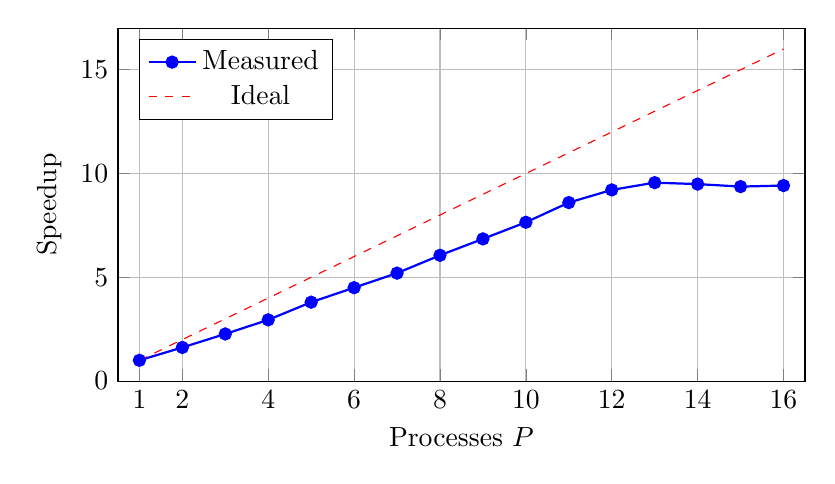
\begin{tikzpicture}
\begin{axis}[
    xlabel={Processes $P$},
    ylabel={Speedup},
    xtick={1,2,4,6,8,10,12,14,16},
    ymin=0, ymax=17,
    xmin=0.5, xmax=16.5,
    grid=major,
    width=0.85\textwidth,
    height=0.5\textwidth,
    legend pos=north west
]
\addplot[blue, thick, mark=*] coordinates {
    (1,1.00) (2,1.62) (3,2.27) (4,2.95) (5,3.80) (6,4.50) (7,5.20) (8,6.06)
    (9,6.85) (10,7.65) (11,8.60) (12,9.21) (13,9.56) (14,9.49) (15,9.37) (16,9.42)
};
\addlegendentry{Measured}
\addplot[red, dashed] coordinates {(1,1) (16,16)};
\addlegendentry{Ideal}
\end{axis}
\end{tikzpicture}
\caption{Speedup vs process count. Ideal linear scaling shown dashed.}
\end{figure}

\begin{figure}[H]
\centering
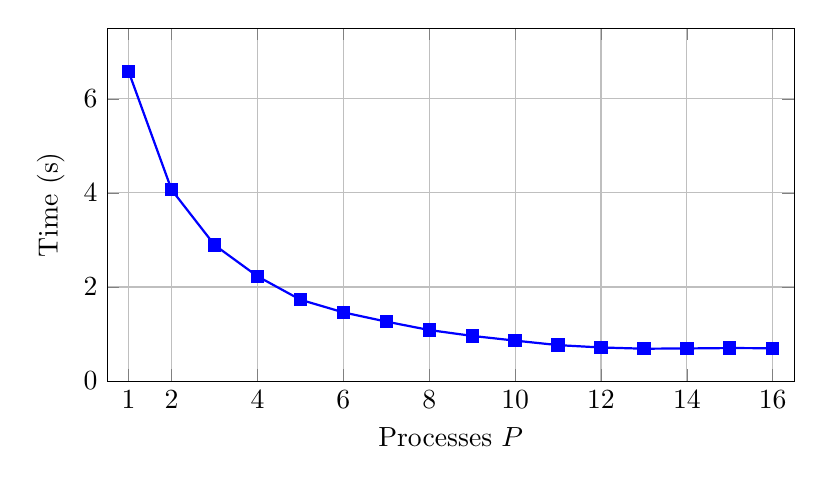
\begin{tikzpicture}
\begin{axis}[
    xlabel={Processes $P$},
    ylabel={Time (s)},
    xtick={1,2,4,6,8,10,12,14,16},
    ymin=0, ymax=7.5,
    xmin=0.5, xmax=16.5,
    grid=major,
    width=0.85\textwidth,
    height=0.5\textwidth
]
\addplot[blue, thick, mark=square*] coordinates {
    (1,6.576) (2,4.066) (3,2.892) (4,2.227) (5,1.729) (6,1.460) (7,1.264) (8,1.085)
    (9,0.960) (10,0.860) (11,0.764) (12,0.714) (13,0.688) (14,0.693) (15,0.702) (16,0.698)
};
\end{axis}
\end{tikzpicture}
\caption{Wall-clock time vs process count.}
\end{figure}

\section{Discussion}

\paragraph{Scaling regime.} Speedup is roughly linear up to about $P=11$, with efficiency staying in the 74--78\% band. This range corresponds to the master--worker scheduler having plenty of long jobs to hand out, so workers rarely idle and the global-bound propagation keeps pruning effective. The $P=1$--$3$ round-robin regime is also efficient (76--81\%) because no rank is wasted on dispatching.

\paragraph{Plateau after $P \approx 12$.} Past 12 processes the speedup flattens around $9.4$--$9.6\times$. Two effects combine: (i) with the master dedicated to scheduling, only $P-1$ ranks compute, so the effective compute count at $P=16$ is 15; (ii) jobs get smaller relative to communication/synchronization overhead and the few long-running jobs become a critical path that additional workers cannot shorten. This is a classic B\&B imbalance: a single heavy subtree serializes the tail of the run regardless of how many idle workers are available.

\paragraph{Correctness.} The output matches the expected answer from the course forum for every $P \in \{1,\ldots,16\}$. Because every rank generates the same job list deterministically and only the scheduling order differs, runs are reproducible up to the choice of which rank happens to discover the winning clique first.

\paragraph{Pseudocode compliance.} The implementation follows Algorithm~1 line-by-line: coloring bound, then knapsack bound, then branch by popping the last candidate, with budget check, $P_{\max}$ update, and neighborhood intersection. The only deviations from a literal transcription are allowed by the instructor's clarifications on Piazza: candidates are pre-sorted once at the top level (by profit/cost ratio) so that the knapsack bound's iteration order is obtained without re-sorting, and the flat adjacency matrix is chosen for cache-friendly $O(1)$ neighbor tests.

\paragraph{Limitations.} \texttt{input\_report.txt} is small enough that even the sequential run finishes in about 6.6 seconds, so the reachable speedup is capped by Amdahl's law as soon as per-job work drops below the MPI message latency. On larger generated graphs (denser or with higher $N$) the plateau moves further right, as expected.

\end{document}
